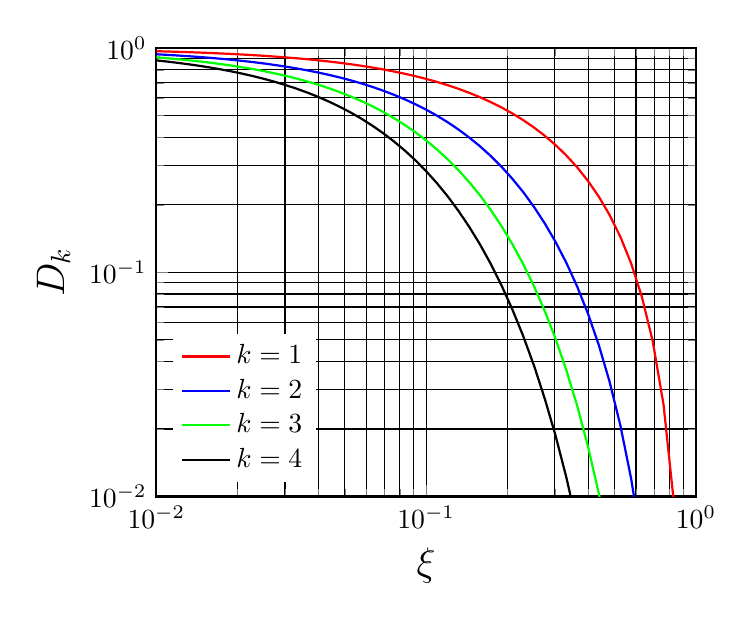
\begin{tikzpicture}
    \pgfplotsset{untmp/.style={domain=0.0001:1,
                              samples=101,
                              unbounded coords=jump,
                              thick}
                }
    \pgfmathsetmacro{\pi}{3.141592653589793}     % dépassement d4 
    \begin{axis}
    [   xmode=log,
        ymode=log,
        legend style={draw=none},
        legend pos=south west,
        axis line style = thick,
        xmin=0.01,
        xmax=1,
        ymin=0.01,
        ymax=1.0,
        xlabel={$\xi$},
        ylabel={$D_k$},
        label style={font=\Large},
        grid=both,
        grid style={line width=.4pt, draw=black},
        major grid style={line width=.4pt,draw=black},
    ]
    \addplot[red,untmp  ] {exp(-(x*\pi)/(sqrt(1-x*x)))};
    \addplot[blue,untmp ] {exp(-(2*x*\pi)/(sqrt(1-x*x)))};
    \addplot[green,untmp] {exp(-(3*x*\pi)/(sqrt(1-x*x)))};
    \addplot[black,untmp] {exp(-(4*x*\pi)/(sqrt(1-x*x)))};
    \legend{$k=1$,$k=2$,$k=3$,$k=4$}
    \end{axis}
\end{tikzpicture}

